\appendix

\section{Additional proof for theorem~\ref{proof1}}
\label{appendix_1}
\textbf{Theorem~\ref{proof1}.} \textit{ERN cannot learn from samples in high uncertainty area.}


\begin{proof}
Consider input $X$ and the corresponding label $y$. We use $\boldsymbol{o}=(o_{\gamma}, o_{v}, o_{\alpha}, o_{\beta})$ to denote the output of $f_{\boldsymbol{\theta}}(X)$.

\textbf{Case I}: $\operatorname{ReLU}(\cdot)$ activation function to get $\alpha$, therefore we have:
\begin{equation}
\begin{aligned}
\alpha&=\operatorname{ReLU}(o_{\alpha}) + 1  \\
      &= \max(0,o_{\alpha})+1 
\end{aligned}
\end{equation}
And,
\begin{equation}
    \frac{\partial \alpha}{\partial o_{\alpha}}=
    \begin{cases}1 & \text { if } \quad o_{\alpha}>0 \\ 
    0 & \text { otherwise }
    \end{cases}
\end{equation}
So the gradient of NLL loss with respect to $o_{\alpha}$ is given by:
\begin{equation}
\begin{aligned}
\frac{\partial \mathcal{L}^{\mathrm{NLL}}}{\partial o_\alpha} &= \frac{\partial \mathcal{L}^{\mathrm{NLL}}}{\partial \alpha} \frac{\partial \alpha}{\partial o_{\alpha}}     \\
&=[\log(1+\frac{\nu(\gamma-y)^2}{2\beta(\nu+1)}) +\psi(\alpha) \\
&- \psi(\alpha+0.5)] \cdot \frac{\partial \alpha}{\partial o_{\alpha}}
\end{aligned}
\end{equation}
where $\psi(\cdot)$ denotes the digamma function.
For a sample in high uncertainty area, we have:
\begin{equation}
    \alpha \rightarrow 1 \Rightarrow o_\alpha <0 \Rightarrow \frac{\partial \alpha}{\partial o_{\alpha}}=0
\end{equation}





\textbf{Case II}: $\operatorname{exp}(\cdot)$ activation function to get $\alpha$, therefore we have:
\begin{equation}
\alpha=\operatorname{exp}(o_{\alpha}) + 1  
\end{equation}
And,
\begin{equation}
    \frac{\partial \alpha}{\partial o_{\alpha}}=\exp(o_{\alpha})
\end{equation}
So the gradient of NLL loss with respect to $o_{\alpha}$ is given by:
\begin{equation}
\begin{aligned}
\frac{\partial \mathcal{L}^{\mathrm{NLL}}}{\partial o_\alpha} &= \frac{\partial \mathcal{L}^{\mathrm{NLL}}}{\partial \alpha} \frac{\partial \alpha}{\partial o_{\alpha}}     \\
&=[\log(1+\frac{\nu(\gamma-y)^2}{2\beta(\nu+1)}) +\psi(\alpha) \\
&- \psi(\alpha+0.5)] \cdot \exp(o_{\alpha})
\end{aligned}
\end{equation}
where $\psi(\cdot)$ denotes the digamma function.

For a sample in high uncertainty area, we have:
\begin{equation}
    \alpha \rightarrow 1 \Rightarrow o_\alpha \rightarrow-\infty \Rightarrow \exp\left(o_\alpha\right) \rightarrow 0
\end{equation}




\textbf{Case III}: $\operatorname{SoftPlus}(\cdot)$ activation function to get $\alpha$, therefore we have:
\begin{equation}
\begin{aligned}
\alpha&=\operatorname{SoftPlus}(o_{\alpha}) + 1  \\
      &= \log(\exp(o_{\alpha})+1)+1 
\end{aligned}
\end{equation}
And,
\begin{equation}
    \frac{\partial \alpha}{\partial o_{\alpha}}=\operatorname{Sigmoid}\left(o_\alpha\right)
\end{equation}
So the gradient of NLL loss with respect to $o_{\alpha}$ is given by:
\begin{equation}
\begin{aligned}
\frac{\partial \mathcal{L}^{\mathrm{NLL}}}{\partial o_\alpha} &= \frac{\partial \mathcal{L}^{\mathrm{NLL}}}{\partial \alpha} \frac{\partial \alpha}{\partial o_{\alpha}}     \\
&=[\log(1+\frac{\nu(\gamma-y)^2}{2\beta(\nu+1)}) +\psi(\alpha) \\
&- \psi(\alpha+0.5)] \cdot \operatorname{Sigmoid}\left(o_\alpha\right)
\end{aligned}
\end{equation}
where $\psi(\cdot)$ denotes the digamma function.

For a sample in high uncertainty area, we have:
\begin{equation}
    \alpha \rightarrow 1 \Rightarrow o_\alpha \rightarrow-\infty \Rightarrow \operatorname{Sigmoid}\left(o_\alpha\right) \rightarrow 0
\end{equation}


Based on the above analysis of \textbf{Case I}, \textbf{Case II} and \textbf{Case III}, for training samples in high uncertainty areas:
\begin{equation}
    \frac{\partial \mathcal{L}^{\mathrm{NLL}}}{\partial o_\alpha} = 0
\end{equation}

And the gradient of $\mathcal{L}^{\mathrm{R}}=|y-\gamma| \cdot(2 v+\alpha)$ with respect to $o_{\alpha}$ is given by:
\begin{equation}
\begin{aligned}
    \frac{\partial \mathcal{L}^{\mathrm{R}}}{\partial o_\alpha}&=\frac{\partial \mathcal{L}^{\mathrm{R}}}{\partial \alpha} \frac{\partial \alpha}{\partial o_\alpha} \\
    &= |y-\gamma| \cdot \frac{\partial \alpha}{\partial o_\alpha}
\end{aligned}
\end{equation}
Similarly, we have:
\begin{equation}
    \frac{\partial \mathcal{L}^{\mathrm{R}}}{\partial o_\alpha} = 0
\end{equation}
And $\mathcal{L}^{\mathrm{ERN}}=\mathcal{L}^{\mathrm{NLL}}+\lambda \mathcal{L}^{\mathrm{R}}$, therefore we have:
\begin{equation}
\begin{aligned}
\frac{\partial \mathcal{L}^{\mathrm{ERN}}}{\partial o_\alpha} &= \frac{\partial \mathcal{L}^{\mathrm{NLL}}}{\partial o_\alpha} +\lambda \frac{\partial \mathcal{L}^{\mathrm{R}}}{\partial o_\alpha} \\
&=0
\end{aligned}
\end{equation}
\end{proof}

Since the gradient of the loss function with respect to $o_{\alpha}$ is zero, there won't be any update on $\alpha$ from such samples. The model fails to learn from samples in high uncertainty area.


\section{Details about experimental setup and additional experiments}
\label{appendix_2}


\subsection{Experimental Setup}
\label{appendix_21}
\subsubsection{Cubic Regression}For Cubic Regression, the problem setup is the same as~\citeauthor{NEURIPS2020_aab08546}.
The training set is composed of examples derived from the cubic equation $y=x^3+\epsilon$, where the error term $\epsilon$ follows a normal distribution $\epsilon \sim \mathcal{N}(0,3)$. We conduct training over the interval $x \in[-4,4]$, and perform testing over $x \in[-6,-4) \cup(4,6]$. All models consisted of 100 neurons with 3 hidden layers and were trained to convergence. The coefficient for $\mathcal{L}^{\mathrm{R}}$ in $\mathcal{L}^{\mathrm{ERN}}$ is $\lambda=0.01$. All models were trained with the Adam optimizer $\eta=5 \mathrm{e}-3$ and a batch size of 128. For experiments within HUA, we give a large negative bias to the activation layer to make the samples fall within HUA at the beginning of training.

\begin{figure}
\centering
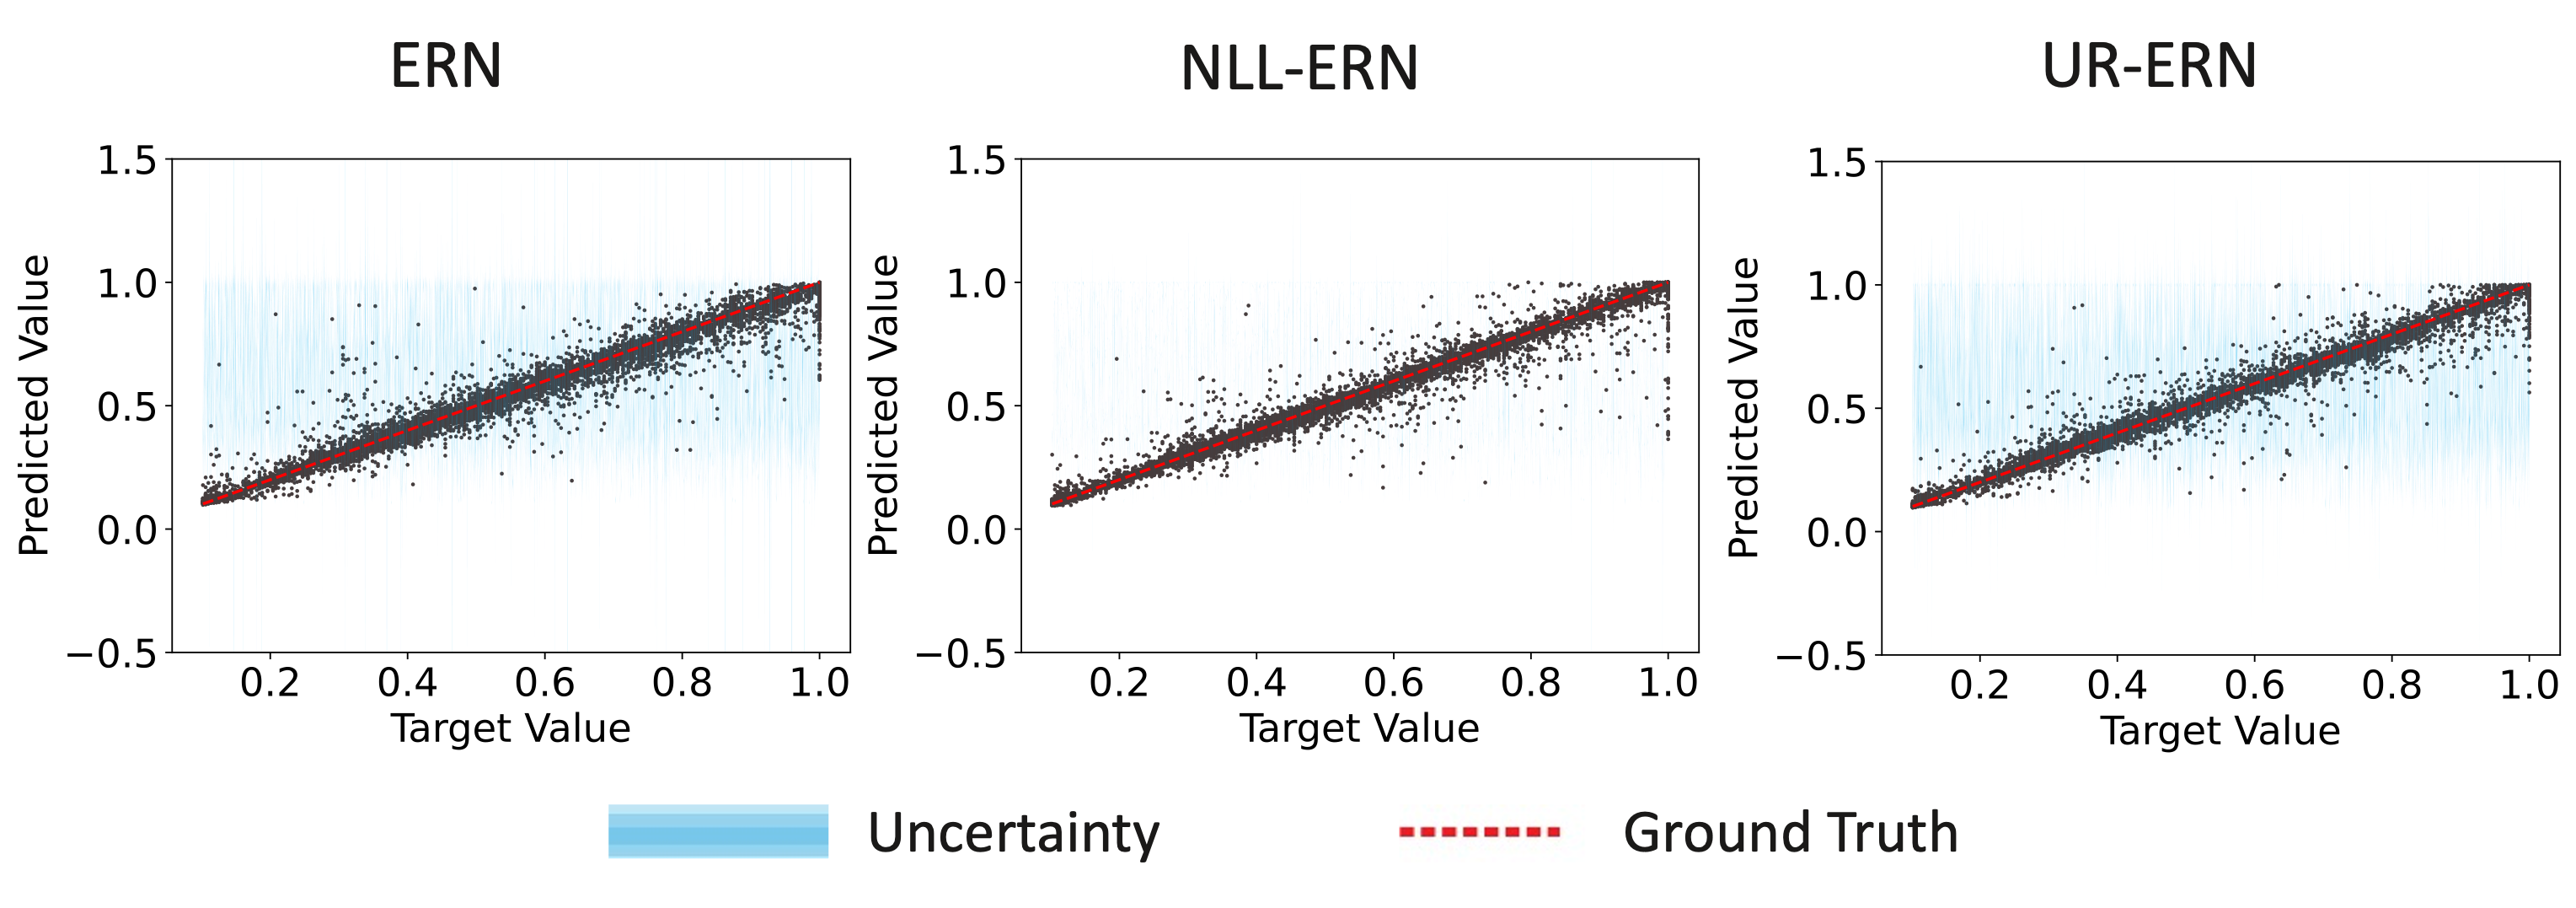
\includegraphics[width=0.9\columnwidth]{depth_outside_HUA_appen.png} 
\caption{Performance of model outside HUA of Depth Estimation. The blue shade represents prediction uncertainty. A good estimation of uncertainty should cover the gap between prediction and ground truth exactly. \ours performs stably well compared with ERN and NLL-ERN both within HUA and outside HUA.}
\label{depth_outside_HUA_appen}
\end{figure}

% \begin{figure}
%     \centering
%         \subfloat[Ground Truth]{
%         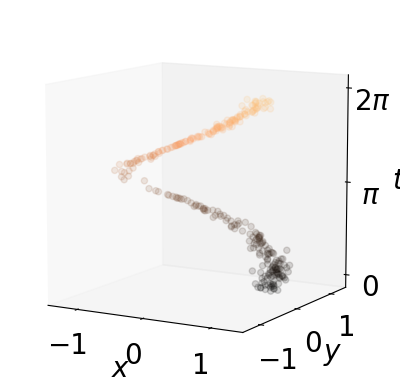
\includegraphics[width=0.45\linewidth]{data.png}
%         %\label{fig:image_cutoff}
%     }
%     \subfloat[Ground Truth]{
%         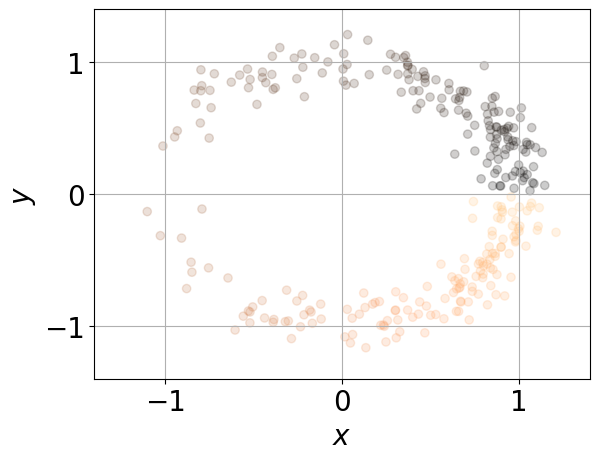
\includegraphics[width=0.45\linewidth]{data_xy.png}
%         %\label{fig:image_cutoff}
%     } \\
%         \subfloat[Multivariate ERN]{
%         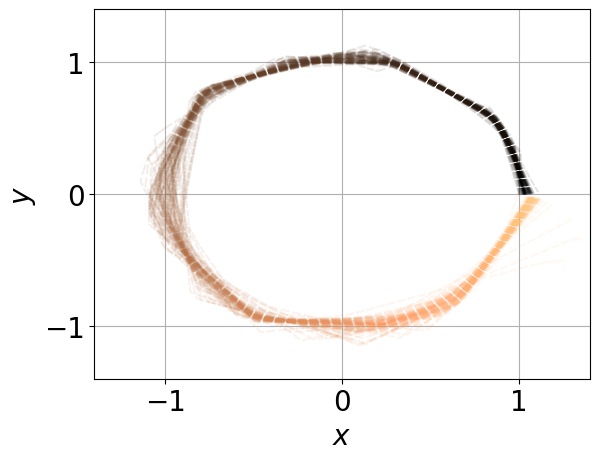
\includegraphics[width=0.45\linewidth]{model_xy_nll.png}
%         %\label{fig:image_calib}
%     }
%     \subfloat[\ours]{
%         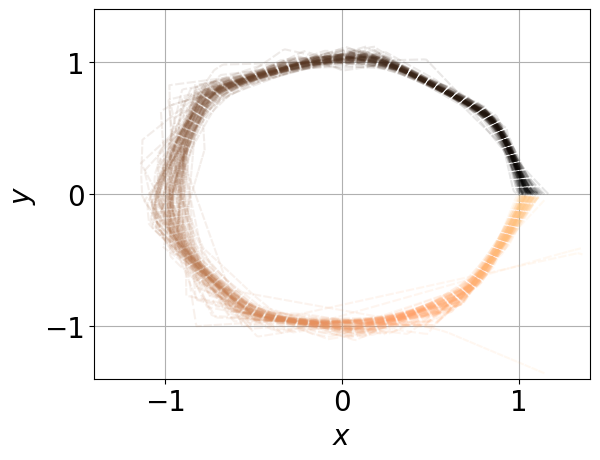
\includegraphics[width=0.45\linewidth]{model_xy.png}
%         %\label{fig:image_calib}
%     }
%     \caption{Prediction of regression target. The value of $t$ is color coded.\hua{can you add explaination to the colors, what does it mean, and what's the conclusion of this figure?}}
%     \label{fig:multivariate_appen}
% \end{figure}

\subsubsection{Depth Estimation}For depth estimation, we also follow the setup of \citeauthor{NEURIPS2020_aab08546}. Depth estimation is conducted on  NYU-Depth-v2 dataset~\cite{silberman2012indoor}. Each image scan's missing depth holes were filled using the Levin Colorization method, and the resulting depth map was inverted to be proportional to disparity, as commonly practiced in depth learning literature. 
The resulting images were saved and used for training a U-Net \cite{ronneberger2015u} backbone model with five convolutional and pooling blocks. The dataset was randomly split into training, validation, and test sets (80-10-10). The input images had a shape of $(160,128)$ with 3 feature maps (RGB), while the target had a single disparity map. 
The training hyperparameters included a batch size of 32, Adam optimization with learning rate $5 \times 10^{-5}$, over 60000 iterations, and $\lambda=0.1$ for ERN. The best model by validation set RMSE was saved for testing. For experiments within HUA, we give a large negative bias to the activation layer to make the samples fall within HUA at the beginning of training.

For out-of-distribution experiments, We use images from ApolloScape \cite{huang2018apolloscape}, an OOD dataset for outdoor driving.

\begin{figure}
    \centering
        \subfloat[Ground Truth]{
        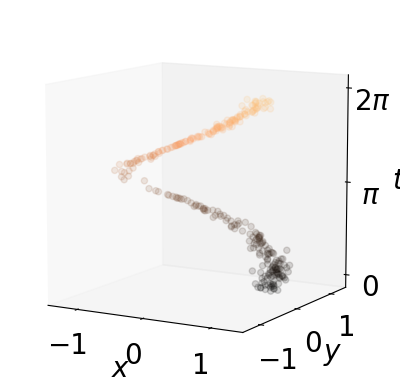
\includegraphics[width=0.45\linewidth]{data.png}
        %\label{fig:image_cutoff}
    }
    \subfloat[Ground Truth ($xy$-plane)]{
        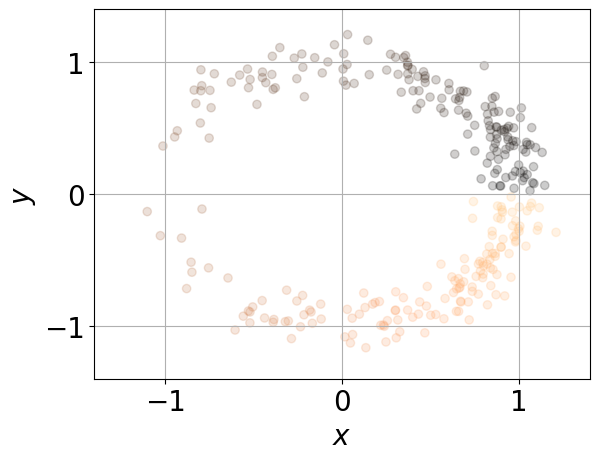
\includegraphics[width=0.45\linewidth]{data_xy.png}
        %\label{fig:image_cutoff}
    } \\
        \subfloat[Multivariate ERN]{
        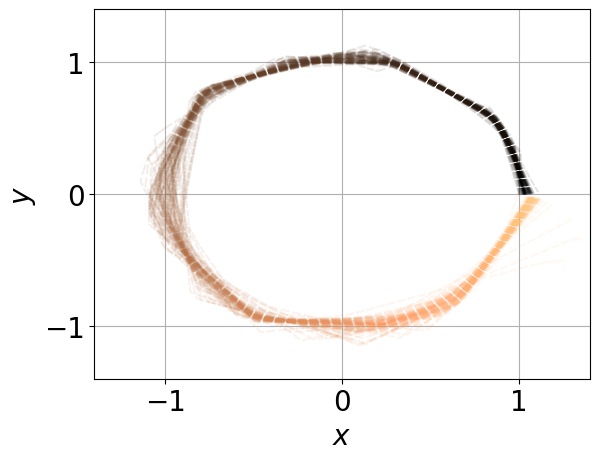
\includegraphics[width=0.45\linewidth]{model_xy_nll.png}
        %\label{fig:image_calib}
    }
    \subfloat[\ours]{
        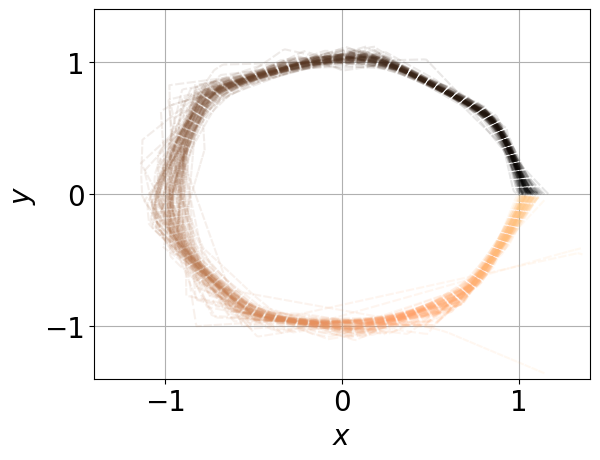
\includegraphics[width=0.45\linewidth]{model_xy.png}
        %\label{fig:image_calib}
    }
    \caption{Prediction of regression target. The value of $t$ is color coded. The larger value of $t$ corresponds to lighter color in the $xy$-plane figures. Besides estimating uncertainty, \ours performs stably well compared with Multivariate ERN in terms of predicting regression targets.}
    \label{fig:multivariate_appen}
\end{figure}




\subsubsection{Multivariate ERN}
For experiments of Multivariate ERN, we follow the setup of \citeauthor{meinert2021multivariate}. The target is to predict $(x, y) \in \mathbb{R}^2$ given $t \in \mathbb{R}$, where $x$ and $y$ being the features of the data sample given input $t$ with the following definition:
\begin{equation}
x=(1+\epsilon) \cos t, \quad 
y=(1+\epsilon) \sin t,
\end{equation}
and the distribution of $t$ is formulated as following:
\begin{equation}
t \sim \begin{cases}1-\frac{\zeta}{\pi} & \text { if } \zeta \in[0, \pi] \\ \frac{\zeta}{\pi}-1 & \text { if } \zeta \in(\pi, 2 \pi] \\ 0 & \text { else }\end{cases}
\end{equation}
where $\zeta \in[0,2 \pi]$ is uniformly distributed and $\epsilon \sim \mathcal{N}(0,0.1)$ is drawn from a normal distribution. We fit a distribution to 300 data points using a small neural network (NN) with one input neuron, two hidden layers of 32 neurons with Rectified Linear Unit activation, and six output neurons. The output $\vec{p} \in \mathbb{R}^6$ is transformed into the parameters of the evidential distribution.:
\begin{equation}
\begin{gathered}
\vec{\mu}=\left(\begin{array}{c}
p_1 \\
p_2
\end{array}\right), \quad \boldsymbol{L}=\left(\begin{array}{cc}
\exp \left\{p_3\right\} & 0 \\
p_4 & \exp \left\{p_5\right\}
\end{array}\right), \\
\nu=8+5 \tanh p_6,
\end{gathered}
\end{equation}
where an exponential function is used to constrain the diagonal elements of $\boldsymbol{L}$ to be strictly positive and the transformation of $\nu$ corresponds to the required lower bound $ \nu>n+1=3$.
All the experiments regarding Multivariate ERN are within HUA, we give a large negative bias to the activation layer to make the samples fall within HUA at the beginning of training.


\begin{figure}
\centering
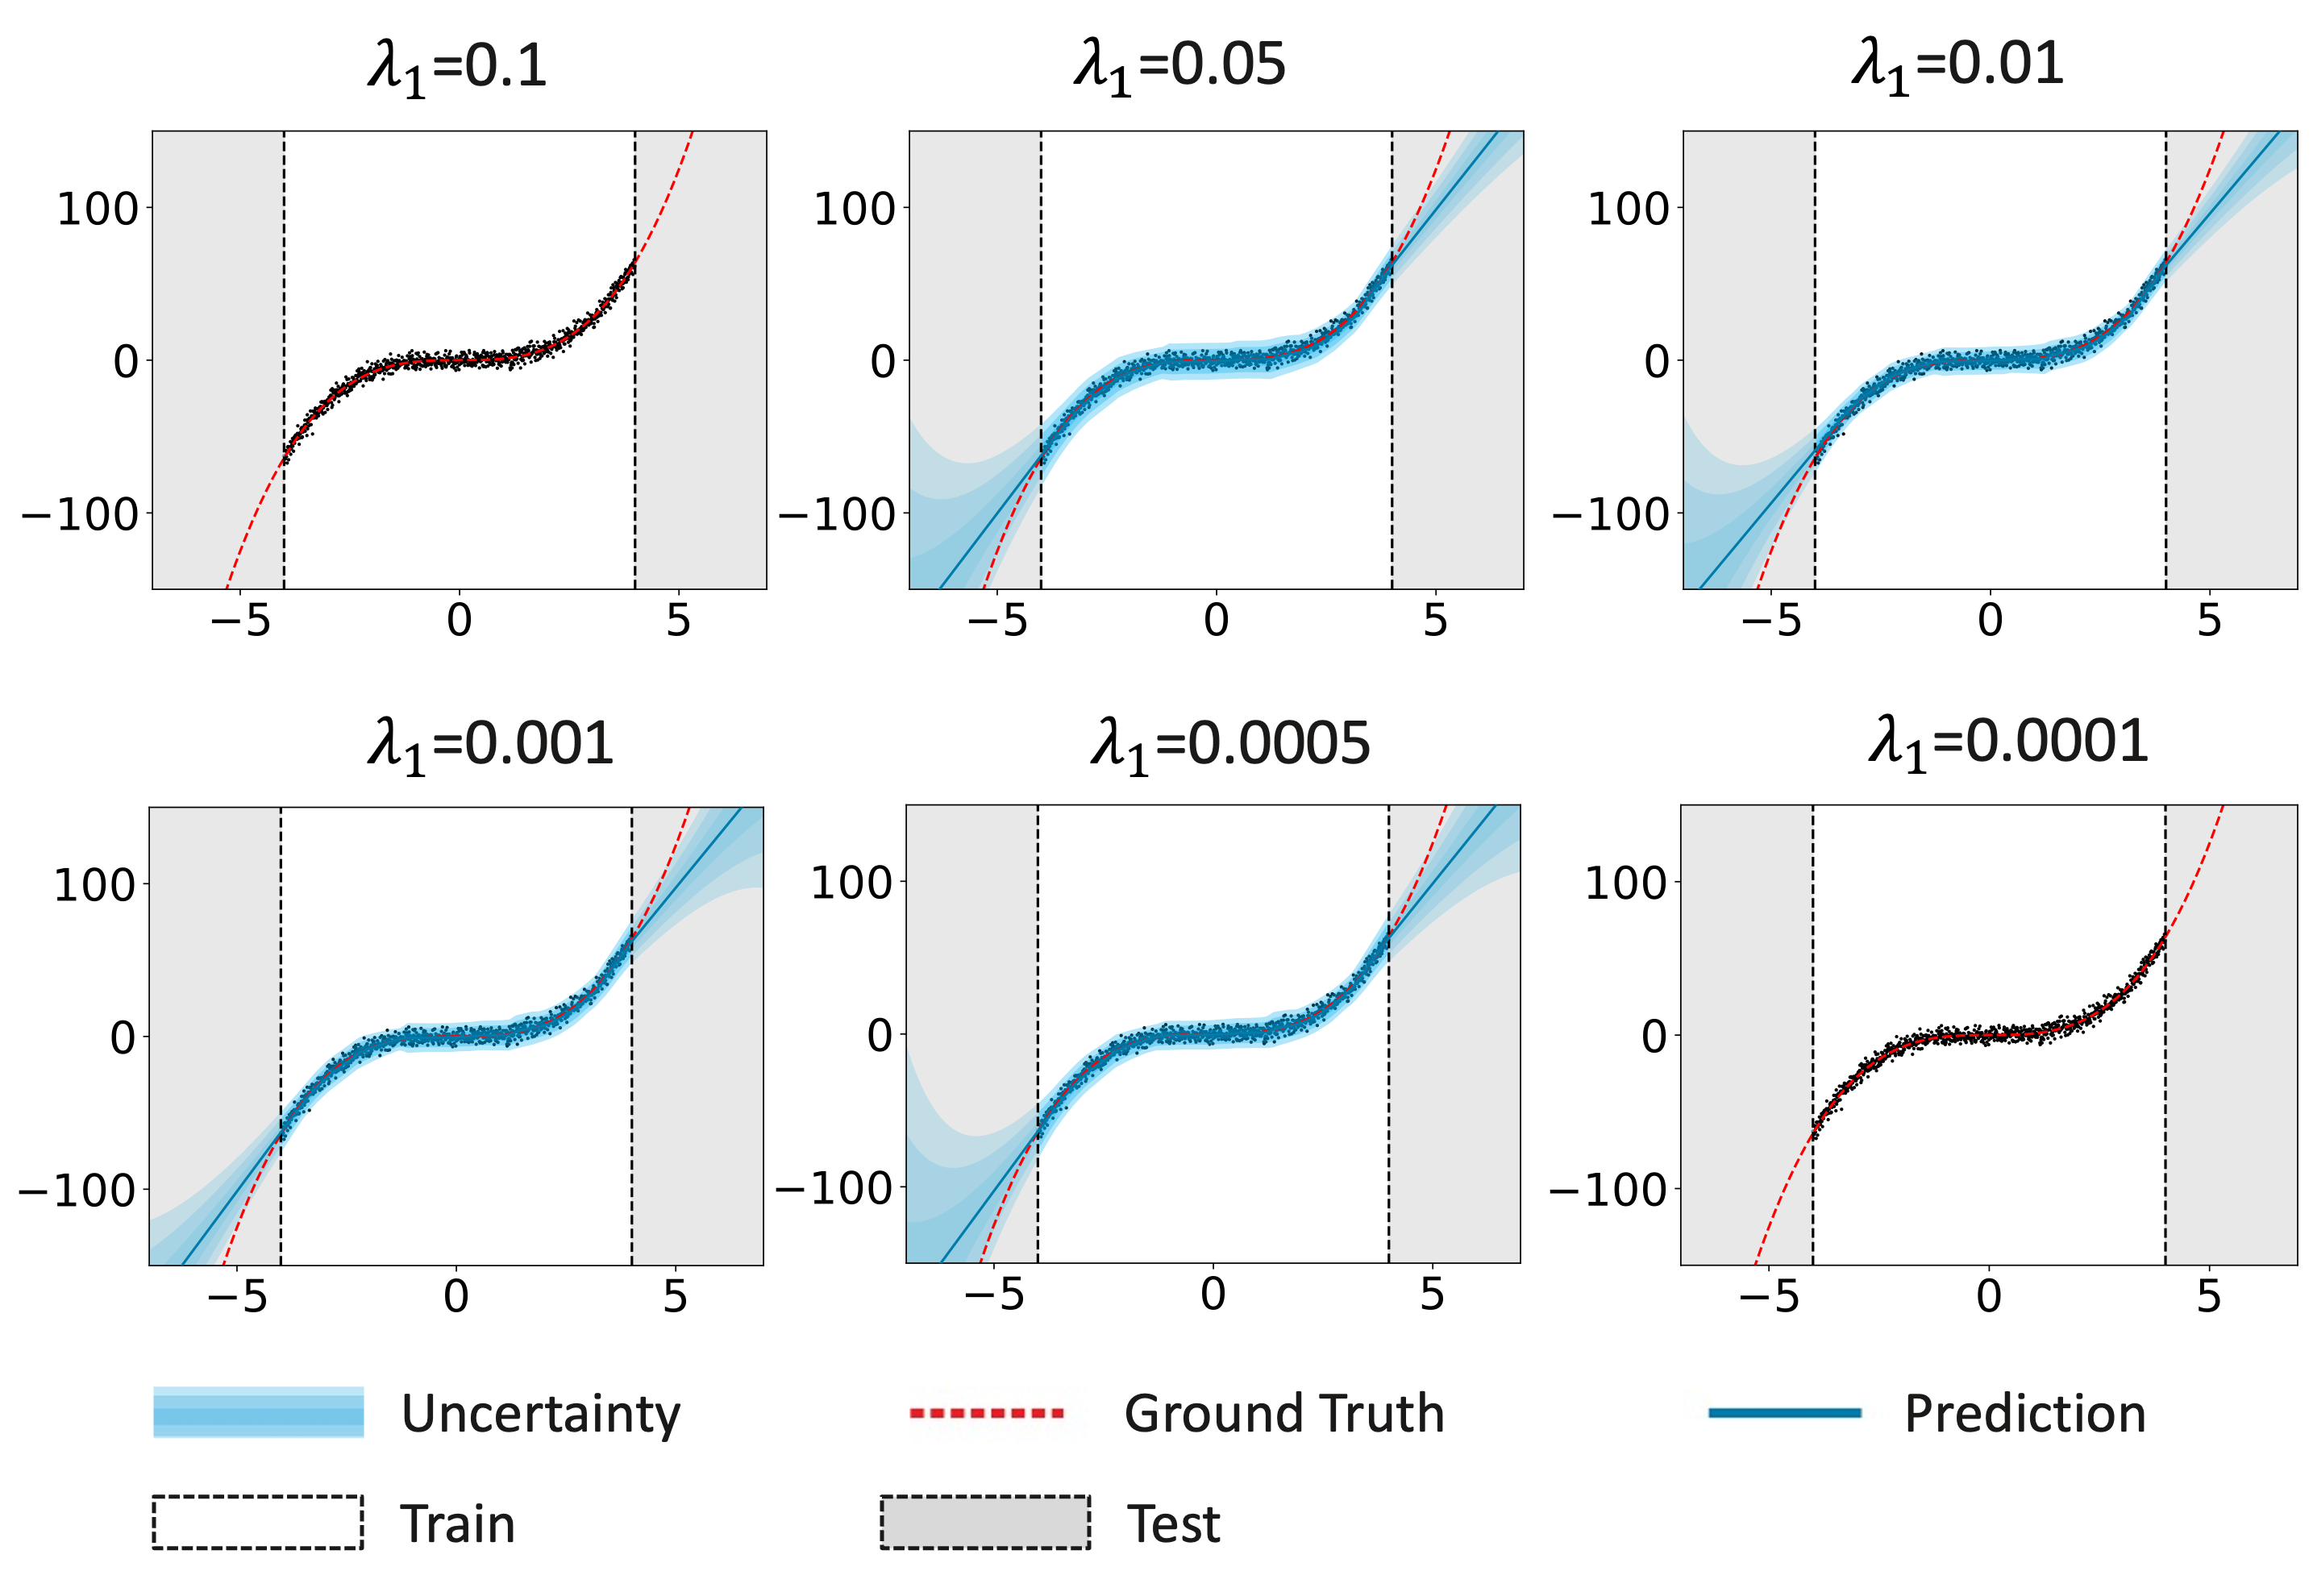
\includegraphics[width=0.9\columnwidth]{sensitivity_outside_HUA.png} 
\caption{Impact of Uncertainty Regularization on model performance. The Figure shows model performance with different coefficients. 
Too small or too large coefficient $\lambda_{1}$ will make the regularization term infinite, failing to correctly estimate uncertainty.}
\label{sensitivity_outside_HUA_appen}
\end{figure}

\subsection{Additional Experiments}
\label{appendix_22}
\subsubsection{Performance on Real-World Benchmark}
We further evaluate the performance of models on the real-world benchmark, the UCI regression dataset \cite{hernandez2015probabilistic}. Our UCI regression experimental setup is the same as \citeauthor{hernandez2015probabilistic} (therefore outside HUA). Following previous works \cite{NEURIPS2020_aab08546,oh2022improving}, we use root mean squared error (RMSE) and negative log-likelihood (NLL) as evaluation metrics.


\begin{table}
\centering
\resizebox{\columnwidth}{!}{%
\begin{tabular}{@{}cccc@{}}
\toprule
\multirow{2}{*}{Datasets} & \multicolumn{3}{c}{RMSE}                                         \\ \cmidrule(l){2-4} 
                          & ERN                 & NLL-ERN             & UR-ERN               \\ \midrule
Boston                    & 3.06(0.16)          & 2.97(0.27)          & \textbf{2.91(0.28)}   \\
Concrete                  & 5.85(0.15)          & 5.76(0.16) & \textbf{5.74(0.24)}           \\
Energy                    & 2.06(0.10)          & 1.93(0.13)          & \textbf{1.88(0.09)}  \\
Kin8nm                    & 0.09(0.00)          & 0.06(0.00)          & \textbf{0.06(0.00)}  \\
Navel                     & 0.00(0.00)          & 0.00(0.00)          & \textbf{0.00(0.00)}  \\
Power                     & 4.23(0.09)          & \textbf{3.01(0.10)} & 3.02(0.08)           \\
Protein                   & 4.64(0.03)          & 3.71(0.15)          & \textbf{3.70(0.15)}  \\
Wine                      & 0.61(0.02)          & 0.57(0.02)          & \textbf{0.56(0.03)}  \\
Yacht                     & 1.57(0.56)          & \textbf{1.38(0.51)} & 1.57(0.54)           \\ \midrule
\multirow{2}{*}{Datasets} & \multicolumn{3}{c}{NLL}                                          \\ \cmidrule(l){2-4} 
                          & ERN                 & NLL-ERN             & UR-ERN               \\ \midrule
Boston                    & 2.35(0.06)          & 2.33(0.06)          & \textbf{2.33(0.06)}  \\
Concrete                  & \textbf{3.01(0.02)} & 3.05(0.03)          & 3.05(0.04)           \\
Energy                    & 1.39(0.06)          & 1.35(0.03)          & \textbf{1.35(0.03)}  \\
Kin8nm                    & -1.24(0.01)         & -1.36(0.03)         & \textbf{-1.37(0.03)} \\
Navel                     & -5.73(0.07)         & -6.24(0.08)         & \textbf{-6.27(0.06)} \\
Power                     & 2.81(0.07)          & \textbf{2.54(0.02)} & 2.55(0.02)           \\
Protein                   & 2.63(0.00)          & \textbf{2.42(0.03)}          & 2.44(0.05)  \\
Wine                      & 0.89(0.05)          & \textbf{0.88(0.04)} & 0.89(0.05)           \\
Yacht                     & 1.03(0.19)          & \textbf{0.98(0.17)} & 1.00(0.15)           \\ \bottomrule
\end{tabular}%
}
\caption{Experimental results on UCI regression benchmark. Following previous works \cite{NEURIPS2020_aab08546,oh2022improving}, we use RMSE and NLL as evaluation metrics.
The best scores are highlighted and we report standard errors in the parentheses. The proposed \ours performs better than ERN and stably well compared with NLL-ERN.
}
\label{tab:UCI}
\end{table}

Table~\ref{tab:UCI} presents the comparison of model performance on UCI regression. As is shown in the table, even outside HUA, \ours still performs better than ERN. NLL-ERN focuses on predicting the target, but it lags behind when estimating uncertainty. Still, \ours performs stably well compared with NLL-ERN on UCI regression benchmark.

We can observe from the UCI regression experiments that the proposed regularization not only helps the model make proper uncertainty estimation but also helps make better predictions of the target (model prediction is $\gamma$). This is not surprising because the gradient of loss function with respect to $\gamma$ is given by (no activation function is applied to $\gamma$):
\begin{equation}
\begin{aligned}
\frac{\partial \mathcal{L}^{\mathrm{NLL}}}{\partial o_\gamma} &=\frac{\partial \mathcal{L}^{\mathrm{NLL}}}{\partial \gamma}  \\
&=\frac{2 \nu\left(\gamma-y_i\right)(\alpha+0.5)}{2 \beta(\nu+1)+\nu\left(\gamma-y_i\right)^2} 
\end{aligned}
\end{equation}
where the parameters ($\gamma, v, \alpha, \beta$) are output of a neural network. If some samples fall in HUA, $\alpha$ will be hard to update, in turn influencing the update of $\gamma$.

\subsubsection{Depth Estimation outside HUA}
% \begin{figure}
% \centering
% 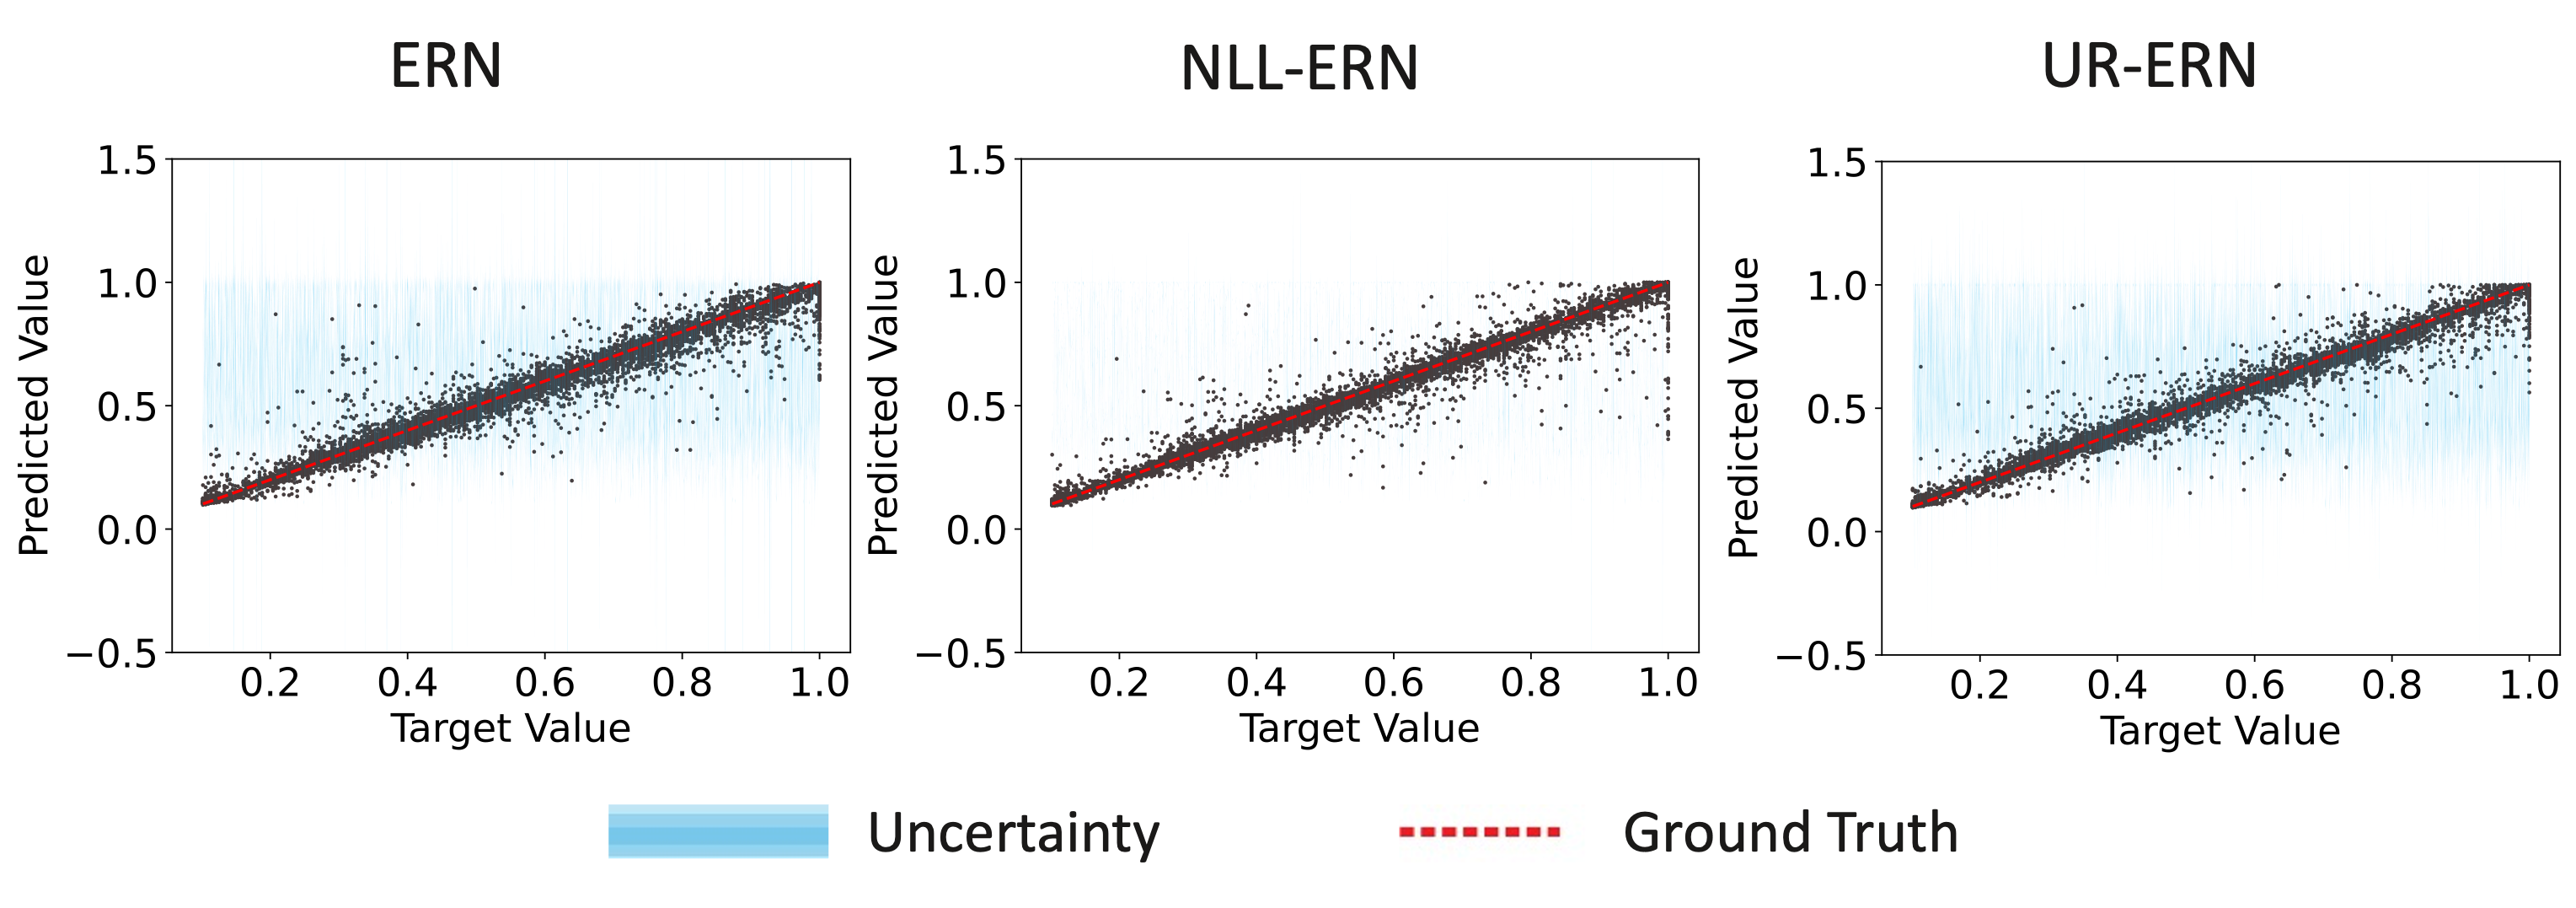
\includegraphics[width=0.9\columnwidth]{depth_outside_HUA_appen.png} 
% \caption{Performance of model outside HUA of Depth Estimation. The blue shade represents prediction uncertainty. A good estimation of uncertainty should cover the gap between prediction and ground truth exactly.}
% \label{depth_outside_HUA_appen}
% \end{figure}
Figure~\ref{depth_outside_HUA_appen} shows the model performance outside HUA. As is shown from the figure, NLL-ERN doesn't perform well in uncertainty estimation, which aligns with the previous study \cite{NEURIPS2020_aab08546}. Compared to the performance  within HUA, ERN performs much better without the problem of zero gradients within HUA. But still, \ours is slightly better than ERN, showing the effectiveness of our method.


\subsubsection{Multivariate ERN}
% \begin{figure}
%     \centering
%     \subfloat[Ground Truth]{
%         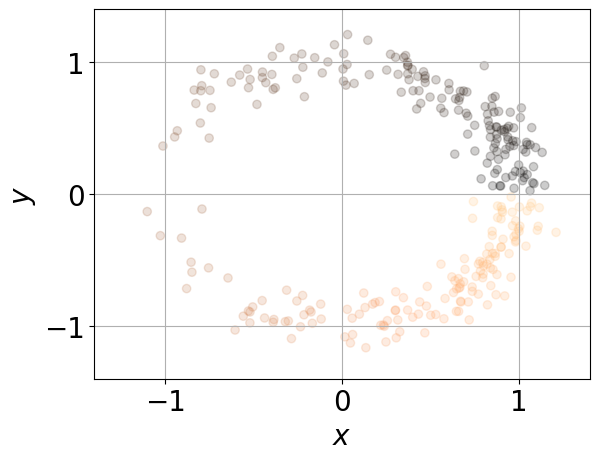
\includegraphics[width=0.3\linewidth]{data_xy.png}
%         %\label{fig:image_cutoff}
%     }
%         \subfloat[Multivariate ERN]{
%         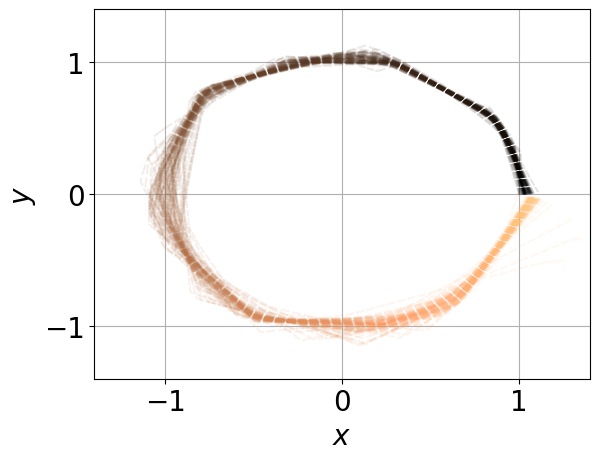
\includegraphics[width=0.3\linewidth]{model_xy_nll.png}
%         %\label{fig:image_calib}
%     }
%     \subfloat[\ours]{
%         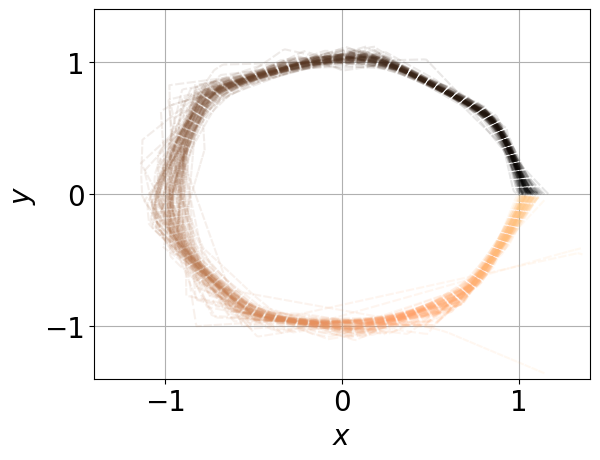
\includegraphics[width=0.3\linewidth]{model_xy.png}
%         %\label{fig:image_calib}
%     }
%     \caption{Prediction of regression target. The value of $t$ is color coded.}
%     \label{fig:multivariate_appen}
% \end{figure}
Figure~\ref{fig:multivariate_appen} shows the prediction of the target for different models. As has been discussed before, we only study $\nu$ (decided by $p_{6}$) in this paper. Therefore, zero gradients of $\nu$ don't affect the prediction of the regression target ($\vec{\mu}$), which can explain the performance in Figure~\ref{fig:multivariate_appen}.

\subsection{Impact of Uncertainty Regularization}
\label{appendix_23}
We conduct experiments on Cubic Regression to investigate the influence of the strength ($\lambda_{1}$) of the proposed Uncertainty Regularization. The sensitivity experiments are conducted with \ours and outside HUA.
By exploring different values for the coefficient $\lambda_{1}$, we assess how the regularization term impacts the model's performance. This analysis helps us understand the sensitivity of our method to this hyperparameter and informs the optimal selection of $\lambda_{1}$ for enhanced uncertainty prediction. 
Figure~\ref{sensitivity_outside_HUA_appen} shows model performance with different coefficients $\lambda_{1}$. As is shown in the Figure, too small or too large coefficient $\lambda_{1}$ will make the regularization term infinite, failing to correctly estimate uncertainty. But if the coefficient is within a certain range, we can see the performance of \ours is pretty stable.